\documentclass[1p]{elsarticle_modified}
%\bibliographystyle{elsarticle-num}

%\usepackage[colorlinks]{hyperref}
%\usepackage{abbrmath_seonhwa} %\Abb, \Ascr, \Acal ,\Abf, \Afrak
\usepackage{amsfonts}
\usepackage{amssymb}
\usepackage{amsmath}
\usepackage{amsthm}
\usepackage{scalefnt}
\usepackage{amsbsy}
\usepackage{kotex}
\usepackage{caption}
\usepackage{subfig}
\usepackage{color}
\usepackage{graphicx}
\usepackage{xcolor} %% white, black, red, green, blue, cyan, magenta, yellow
\usepackage{float}
\usepackage{setspace}
\usepackage{hyperref}

\usepackage{tikz}
\usetikzlibrary{arrows}

\usepackage{multirow}
\usepackage{array} % fixed length table
\usepackage{hhline}

%%%%%%%%%%%%%%%%%%%%%
\makeatletter
\renewcommand*\env@matrix[1][\arraystretch]{%
	\edef\arraystretch{#1}%
	\hskip -\arraycolsep
	\let\@ifnextchar\new@ifnextchar
	\array{*\c@MaxMatrixCols c}}
\makeatother %https://tex.stackexchange.com/questions/14071/how-can-i-increase-the-line-spacing-in-a-matrix
%%%%%%%%%%%%%%%

\usepackage[normalem]{ulem}

\newcommand{\msout}[1]{\ifmmode\text{\sout{\ensuremath{#1}}}\else\sout{#1}\fi}
%SOURCE: \msout is \stkout macro in https://tex.stackexchange.com/questions/20609/strikeout-in-math-mode

\newcommand{\cancel}[1]{
	\ifmmode
	{\color{red}\msout{#1}}
	\else
	{\color{red}\sout{#1}}
	\fi
}

\newcommand{\add}[1]{
	{\color{blue}\uwave{#1}}
}

\newcommand{\replace}[2]{
	\ifmmode
	{\color{red}\msout{#1}}{\color{blue}\uwave{#2}}
	\else
	{\color{red}\sout{#1}}{\color{blue}\uwave{#2}}
	\fi
}

\newcommand{\Sol}{\mathcal{S}} %segment
\newcommand{\D}{D} %diagram
\newcommand{\A}{\mathcal{A}} %arc


%%%%%%%%%%%%%%%%%%%%%%%%%%%%%5 test

\def\sl{\operatorname{\textup{SL}}(2,\Cbb)}
\def\psl{\operatorname{\textup{PSL}}(2,\Cbb)}
\def\quan{\mkern 1mu \triangleright \mkern 1mu}

\theoremstyle{definition}
\newtheorem{thm}{Theorem}[section]
\newtheorem{prop}[thm]{Proposition}
\newtheorem{lem}[thm]{Lemma}
\newtheorem{ques}[thm]{Question}
\newtheorem{cor}[thm]{Corollary}
\newtheorem{defn}[thm]{Definition}
\newtheorem{exam}[thm]{Example}
\newtheorem{rmk}[thm]{Remark}
\newtheorem{alg}[thm]{Algorithm}

\newcommand{\I}{\sqrt{-1}}
\begin{document}

%\begin{frontmatter}
%
%\title{Boundary parabolic representations of knots up to 8 crossings}
%
%%% Group authors per affiliation:
%\author{Yunhi Cho} 
%\address{Department of Mathematics, University of Seoul, Seoul, Korea}
%\ead{yhcho@uos.ac.kr}
%
%
%\author{Seonhwa Kim} %\fnref{s_kim}}
%\address{Center for Geometry and Physics, Institute for Basic Science, Pohang, 37673, Korea}
%\ead{ryeona17@ibs.re.kr}
%
%\author{Hyuk Kim}
%\address{Department of Mathematical Sciences, Seoul National University, Seoul 08826, Korea}
%\ead{hyukkim@snu.ac.kr}
%
%\author{Seokbeom Yoon}
%\address{Department of Mathematical Sciences, Seoul National University, Seoul, 08826,  Korea}
%\ead{sbyoon15@snu.ac.kr}
%
%\begin{abstract}
%We find all boundary parabolic representation of knots up to 8 crossings.
%
%\end{abstract}
%\begin{keyword}
%    \MSC[2010] 57M25 
%\end{keyword}
%
%\end{frontmatter}

%\linenumbers
%\tableofcontents
%
\newcommand\colored[1]{\textcolor{white}{\rule[-0.35ex]{0.8em}{1.4ex}}\kern-0.8em\color{red} #1}%
%\newcommand\colored[1]{\textcolor{white}{ #1}\kern-2.17ex	\textcolor{white}{ #1}\kern-1.81ex	\textcolor{white}{ #1}\kern-2.15ex\color{red}#1	}

{\Large $\underline{12a_{0646}~(K12a_{0646})}$}

\setlength{\tabcolsep}{10pt}
\renewcommand{\arraystretch}{1.6}
\vspace{1cm}\begin{tabular}{m{100pt}>{\centering\arraybackslash}m{274pt}}
\multirow{5}{120pt}{
	\centering
	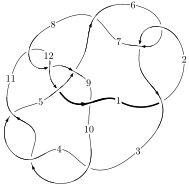
\includegraphics[width=112pt]{../../../GIT/diagram.site/Diagrams/png/1447_12a_0646.png}\\
\ \ \ A knot diagram\footnotemark}&
\allowdisplaybreaks
\textbf{Linearized knot diagam} \\
\cline{2-2}
 &
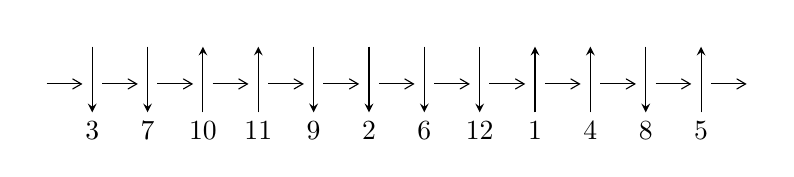
\begin{tikzpicture}[x=20pt, y=17pt]
	% nodes
	\node (C0) at (0, 0) {};
	\node (C1) at (1, 0) {};
	\node (C1U) at (1, +1) {};
	\node (C1D) at (1, -1) {3};

	\node (C2) at (2, 0) {};
	\node (C2U) at (2, +1) {};
	\node (C2D) at (2, -1) {7};

	\node (C3) at (3, 0) {};
	\node (C3U) at (3, +1) {};
	\node (C3D) at (3, -1) {10};

	\node (C4) at (4, 0) {};
	\node (C4U) at (4, +1) {};
	\node (C4D) at (4, -1) {11};

	\node (C5) at (5, 0) {};
	\node (C5U) at (5, +1) {};
	\node (C5D) at (5, -1) {9};

	\node (C6) at (6, 0) {};
	\node (C6U) at (6, +1) {};
	\node (C6D) at (6, -1) {2};

	\node (C7) at (7, 0) {};
	\node (C7U) at (7, +1) {};
	\node (C7D) at (7, -1) {6};

	\node (C8) at (8, 0) {};
	\node (C8U) at (8, +1) {};
	\node (C8D) at (8, -1) {12};

	\node (C9) at (9, 0) {};
	\node (C9U) at (9, +1) {};
	\node (C9D) at (9, -1) {1};

	\node (C10) at (10, 0) {};
	\node (C10U) at (10, +1) {};
	\node (C10D) at (10, -1) {4};

	\node (C11) at (11, 0) {};
	\node (C11U) at (11, +1) {};
	\node (C11D) at (11, -1) {8};

	\node (C12) at (12, 0) {};
	\node (C12U) at (12, +1) {};
	\node (C12D) at (12, -1) {5};
	\node (C13) at (13, 0) {};

	% arrows
	\draw[->,>={angle 60}]
	(C0) edge (C1) (C1) edge (C2) (C2) edge (C3) (C3) edge (C4) (C4) edge (C5) (C5) edge (C6) (C6) edge (C7) (C7) edge (C8) (C8) edge (C9) (C9) edge (C10) (C10) edge (C11) (C11) edge (C12) (C12) edge (C13) ;	\draw[->,>=stealth]
	(C1U) edge (C1D) (C2U) edge (C2D) (C3D) edge (C3U) (C4D) edge (C4U) (C5U) edge (C5D) (C6U) edge (C6D) (C7U) edge (C7D) (C8U) edge (C8D) (C9D) edge (C9U) (C10D) edge (C10U) (C11U) edge (C11D) (C12D) edge (C12U) ;
	\end{tikzpicture} \\
\hhline{~~} \\& 
\textbf{Solving Sequence} \\ \cline{2-2} 
 &
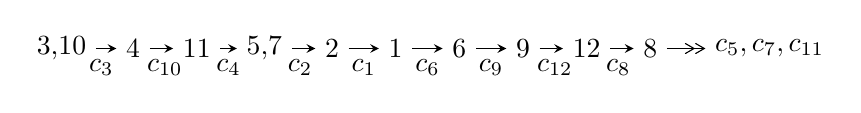
\begin{tikzpicture}[x=23pt, y=7pt]
	% node
	\node (A0) at (-1/8, 0) {3,10};
	\node (A1) at (1, 0) {4};
	\node (A2) at (2, 0) {11};
	\node (A3) at (49/16, 0) {5,7};
	\node (A4) at (33/8, 0) {2};
	\node (A5) at (41/8, 0) {1};
	\node (A6) at (49/8, 0) {6};
	\node (A7) at (57/8, 0) {9};
	\node (A8) at (65/8, 0) {12};
	\node (A9) at (73/8, 0) {8};
	\node (C1) at (1/2, -1) {$c_{3}$};
	\node (C2) at (3/2, -1) {$c_{10}$};
	\node (C3) at (5/2, -1) {$c_{4}$};
	\node (C4) at (29/8, -1) {$c_{2}$};
	\node (C5) at (37/8, -1) {$c_{1}$};
	\node (C6) at (45/8, -1) {$c_{6}$};
	\node (C7) at (53/8, -1) {$c_{9}$};
	\node (C8) at (61/8, -1) {$c_{12}$};
	\node (C9) at (69/8, -1) {$c_{8}$};
	\node (A10) at (11, 0) {$c_{5},c_{7},c_{11}$};

	% edge
	\draw[->,>=stealth]	
	(A0) edge (A1) (A1) edge (A2) (A2) edge (A3) (A3) edge (A4) (A4) edge (A5) (A5) edge (A6) (A6) edge (A7) (A7) edge (A8) (A8) edge (A9) ;
	\draw[->>,>={angle 60}]	
	(A9) edge (A10);
\end{tikzpicture} \\ 

\end{tabular} \\

\footnotetext{
The image of knot diagram is generated by the software ``\textbf{Draw programme}" developed by Andrew Bartholomew(\url{http://www.layer8.co.uk/maths/draw/index.htm\#Running-draw}), where we modified some parts for our purpose(\url{https://github.com/CATsTAILs/LinksPainter}).
}\phantom \\ \newline 
\centering \textbf{Ideals for irreducible components\footnotemark of $X_{\text{par}}$} 
 
\begin{align*}
I^u_{1}&=\langle 
-7.92758\times10^{283} u^{107}+4.71823\times10^{283} u^{106}+\cdots+3.98501\times10^{285} b-7.76087\times10^{285},\\
\phantom{I^u_{1}}&\phantom{= \langle  }1.13273\times10^{285} u^{107}-9.80011\times10^{284} u^{106}+\cdots+3.98501\times10^{285} a+4.87210\times10^{286},\\
\phantom{I^u_{1}}&\phantom{= \langle  }u^{108}- u^{107}+\cdots+26 u-11\rangle \\
I^u_{2}&=\langle 
2 u^{22}-25 u^{20}+\cdots+b+1,\;u^{22}- u^{21}+\cdots+3 u^2+a,\;u^{24}-14 u^{22}+\cdots-2 u-1\rangle \\
\\
\end{align*}
\raggedright * 2 irreducible components of $\dim_{\mathbb{C}}=0$, with total 132 representations.\\
\footnotetext{All coefficients of polynomials are rational numbers. But the coefficients are sometimes approximated in decimal forms when there is not enough margin.}
\newpage
\renewcommand{\arraystretch}{1}
\centering \section*{I. $I^u_{1}= \langle -7.93\times10^{283} u^{107}+4.72\times10^{283} u^{106}+\cdots+3.99\times10^{285} b-7.76\times10^{285},\;1.13\times10^{285} u^{107}-9.80\times10^{284} u^{106}+\cdots+3.99\times10^{285} a+4.87\times10^{286},\;u^{108}- u^{107}+\cdots+26 u-11 \rangle$}
\flushleft \textbf{(i) Arc colorings}\\
\begin{tabular}{m{7pt} m{180pt} m{7pt} m{180pt} }
\flushright $a_{3}=$&$\begin{pmatrix}1\\0\end{pmatrix}$ \\
\flushright $a_{10}=$&$\begin{pmatrix}0\\u\end{pmatrix}$ \\
\flushright $a_{4}=$&$\begin{pmatrix}1\\- u^2\end{pmatrix}$ \\
\flushright $a_{11}=$&$\begin{pmatrix}u\\- u^3+u\end{pmatrix}$ \\
\flushright $a_{5}=$&$\begin{pmatrix}- u^2+1\\u^4-2 u^2\end{pmatrix}$ \\
\flushright $a_{7}=$&$\begin{pmatrix}-0.284248 u^{107}+0.245924 u^{106}+\cdots+10.9026 u-12.2261\\0.0198935 u^{107}-0.0118399 u^{106}+\cdots+2.17302 u+1.94751\end{pmatrix}$ \\
\flushright $a_{2}=$&$\begin{pmatrix}0.360690 u^{107}-0.270251 u^{106}+\cdots+1.54015 u+9.66541\\-0.0900518 u^{107}+0.0775866 u^{106}+\cdots-0.158843 u-3.11708\end{pmatrix}$ \\
\flushright $a_{1}=$&$\begin{pmatrix}0.270638 u^{107}-0.192664 u^{106}+\cdots+1.38131 u+6.54832\\-0.0900518 u^{107}+0.0775866 u^{106}+\cdots-0.158843 u-3.11708\end{pmatrix}$ \\
\flushright $a_{6}=$&$\begin{pmatrix}0.148781 u^{107}-0.120193 u^{106}+\cdots+22.8571 u-8.84548\\-0.103904 u^{107}+0.0906090 u^{106}+\cdots+1.01686 u+0.660943\end{pmatrix}$ \\
\flushright $a_{9}=$&$\begin{pmatrix}-0.145309 u^{107}+0.0890517 u^{106}+\cdots+65.6658 u-1.78163\\0.0984535 u^{107}-0.0925638 u^{106}+\cdots-10.1060 u+1.78977\end{pmatrix}$ \\
\flushright $a_{12}=$&$\begin{pmatrix}0.320127 u^{107}-0.229063 u^{106}+\cdots-2.02885 u+7.86571\\-0.0950938 u^{107}+0.0815686 u^{106}+\cdots-0.615292 u-3.45990\end{pmatrix}$ \\
\flushright $a_{8}=$&$\begin{pmatrix}0.260853 u^{107}-0.268189 u^{106}+\cdots+21.6743 u+5.87060\\-0.0436157 u^{107}+0.0722231 u^{106}+\cdots-6.07149 u-0.742645\end{pmatrix}$\\&\end{tabular}
\flushleft \textbf{(ii) Obstruction class $= -1$}\\~\\
\flushleft \textbf{(iii) Cusp Shapes $= 0.846668 u^{107}-0.481174 u^{106}+\cdots-26.5586 u+18.7422$}\\~\\
\newpage\renewcommand{\arraystretch}{1}
\flushleft \textbf{(iv) u-Polynomials at the component}\newline \\
\begin{tabular}{m{50pt}|m{274pt}}
Crossings & \hspace{64pt}u-Polynomials at each crossing \\
\hline $$\begin{aligned}c_{1},c_{7}\end{aligned}$$&$\begin{aligned}
&u^{108}+33 u^{107}+\cdots+2423 u+49
\end{aligned}$\\
\hline $$\begin{aligned}c_{2},c_{6}\end{aligned}$$&$\begin{aligned}
&u^{108}- u^{107}+\cdots+57 u+7
\end{aligned}$\\
\hline $$\begin{aligned}c_{3},c_{4},c_{10}\end{aligned}$$&$\begin{aligned}
&u^{108}+u^{107}+\cdots-26 u-11
\end{aligned}$\\
\hline $$\begin{aligned}c_{5}\end{aligned}$$&$\begin{aligned}
&u^{108}-2 u^{107}+\cdots-5 u-1
\end{aligned}$\\
\hline $$\begin{aligned}c_{8},c_{11}\end{aligned}$$&$\begin{aligned}
&u^{108}- u^{107}+\cdots-20 u-1
\end{aligned}$\\
\hline $$\begin{aligned}c_{9}\end{aligned}$$&$\begin{aligned}
&u^{108}-7 u^{107}+\cdots-23253384 u+9157221
\end{aligned}$\\
\hline $$\begin{aligned}c_{12}\end{aligned}$$&$\begin{aligned}
&u^{108}-4 u^{107}+\cdots-46 u+1
\end{aligned}$\\
\hline
\end{tabular}\\~\\
\newpage\renewcommand{\arraystretch}{1}
\flushleft \textbf{(v) Riley Polynomials at the component}\newline \\
\begin{tabular}{m{50pt}|m{274pt}}
Crossings & \hspace{64pt}Riley Polynomials at each crossing \\
\hline $$\begin{aligned}c_{1},c_{7}\end{aligned}$$&$\begin{aligned}
&y^{108}+95 y^{107}+\cdots+121085 y+2401
\end{aligned}$\\
\hline $$\begin{aligned}c_{2},c_{6}\end{aligned}$$&$\begin{aligned}
&y^{108}-33 y^{107}+\cdots-2423 y+49
\end{aligned}$\\
\hline $$\begin{aligned}c_{3},c_{4},c_{10}\end{aligned}$$&$\begin{aligned}
&y^{108}-115 y^{107}+\cdots-8530 y+121
\end{aligned}$\\
\hline $$\begin{aligned}c_{5}\end{aligned}$$&$\begin{aligned}
&y^{108}-2 y^{107}+\cdots-361 y+1
\end{aligned}$\\
\hline $$\begin{aligned}c_{8},c_{11}\end{aligned}$$&$\begin{aligned}
&y^{108}-59 y^{107}+\cdots-86 y+1
\end{aligned}$\\
\hline $$\begin{aligned}c_{9}\end{aligned}$$&$\begin{aligned}
&y^{108}-43 y^{107}+\cdots-3544469265509532 y+83854696442841
\end{aligned}$\\
\hline $$\begin{aligned}c_{12}\end{aligned}$$&$\begin{aligned}
&y^{108}-6 y^{107}+\cdots-2902 y+1
\end{aligned}$\\
\hline
\end{tabular}\\~\\
\newpage\flushleft \textbf{(vi) Complex Volumes and Cusp Shapes}
$$\begin{array}{c|c|c}  
\text{Solutions to }I^u_{1}& \I (\text{vol} + \sqrt{-1}CS) & \text{Cusp shape}\\
 \hline 
\begin{aligned}
u &= -0.826406 + 0.702326 I \\
a &= \phantom{-}0.296844 - 0.632579 I \\
b &= \phantom{-}0.892571 - 0.164092 I\end{aligned}
 & -3.58745 + 2.67889 I & \phantom{-0.000000 } 0 \\ \hline\begin{aligned}
u &= -0.826406 - 0.702326 I \\
a &= \phantom{-}0.296844 + 0.632579 I \\
b &= \phantom{-}0.892571 + 0.164092 I\end{aligned}
 & -3.58745 - 2.67889 I & \phantom{-0.000000 } 0 \\ \hline\begin{aligned}
u &= \phantom{-}0.657589 + 0.874313 I \\
a &= -0.407294 - 0.511888 I \\
b &= \phantom{-}0.756612 + 0.854103 I\end{aligned}
 & \phantom{-}2.61583 + 6.87570 I & \phantom{-0.000000 } 0 \\ \hline\begin{aligned}
u &= \phantom{-}0.657589 - 0.874313 I \\
a &= -0.407294 + 0.511888 I \\
b &= \phantom{-}0.756612 - 0.854103 I\end{aligned}
 & \phantom{-}2.61583 - 6.87570 I & \phantom{-0.000000 } 0 \\ \hline\begin{aligned}
u &= -1.052110 + 0.317805 I \\
a &= \phantom{-}0.61143 + 1.83434 I \\
b &= -0.916488 - 0.526739 I\end{aligned}
 & -1.62328 - 1.93773 I & \phantom{-0.000000 } 0 \\ \hline\begin{aligned}
u &= -1.052110 - 0.317805 I \\
a &= \phantom{-}0.61143 - 1.83434 I \\
b &= -0.916488 + 0.526739 I\end{aligned}
 & -1.62328 + 1.93773 I & \phantom{-0.000000 } 0 \\ \hline\begin{aligned}
u &= -0.613248 + 0.934669 I \\
a &= \phantom{-}0.61329 - 1.40339 I \\
b &= \phantom{-}1.000230 + 0.772968 I\end{aligned}
 & \phantom{-}1.86526 - 12.94090 I & \phantom{-0.000000 } 0 \\ \hline\begin{aligned}
u &= -0.613248 - 0.934669 I \\
a &= \phantom{-}0.61329 + 1.40339 I \\
b &= \phantom{-}1.000230 - 0.772968 I\end{aligned}
 & \phantom{-}1.86526 + 12.94090 I & \phantom{-0.000000 } 0 \\ \hline\begin{aligned}
u &= -0.594600 + 0.640184 I \\
a &= -0.695431 + 0.121637 I \\
b &= \phantom{-}0.812998 - 0.817444 I\end{aligned}
 & \phantom{-}5.54210 - 1.30136 I & \phantom{-0.000000 } 0 \\ \hline\begin{aligned}
u &= -0.594600 - 0.640184 I \\
a &= -0.695431 - 0.121637 I \\
b &= \phantom{-}0.812998 + 0.817444 I\end{aligned}
 & \phantom{-}5.54210 + 1.30136 I & \phantom{-0.000000 } 0\\
 \hline 
 \end{array}$$\newpage$$\begin{array}{c|c|c}  
\text{Solutions to }I^u_{1}& \I (\text{vol} + \sqrt{-1}CS) & \text{Cusp shape}\\
 \hline 
\begin{aligned}
u &= -0.397084 + 0.760441 I \\
a &= -1.085940 + 0.411506 I \\
b &= -1.054780 - 0.256957 I\end{aligned}
 & -4.74558 - 7.66662 I & \phantom{-0.000000 } 0 \\ \hline\begin{aligned}
u &= -0.397084 - 0.760441 I \\
a &= -1.085940 - 0.411506 I \\
b &= -1.054780 + 0.256957 I\end{aligned}
 & -4.74558 + 7.66662 I & \phantom{-0.000000 } 0 \\ \hline\begin{aligned}
u &= \phantom{-}0.527829 + 0.671958 I \\
a &= \phantom{-}1.08421 + 1.68069 I \\
b &= \phantom{-}0.952806 - 0.776200 I\end{aligned}
 & \phantom{-}5.11087 + 7.27382 I & \phantom{-0.000000 } 0 \\ \hline\begin{aligned}
u &= \phantom{-}0.527829 - 0.671958 I \\
a &= \phantom{-}1.08421 - 1.68069 I \\
b &= \phantom{-}0.952806 + 0.776200 I\end{aligned}
 & \phantom{-}5.11087 - 7.27382 I & \phantom{-0.000000 } 0 \\ \hline\begin{aligned}
u &= \phantom{-}0.846524 + 0.076552 I \\
a &= \phantom{-}0.51787 + 2.49500 I \\
b &= -0.685420 - 0.532665 I\end{aligned}
 & -0.84832 - 2.31753 I & \phantom{-0.000000 } 0 \\ \hline\begin{aligned}
u &= \phantom{-}0.846524 - 0.076552 I \\
a &= \phantom{-}0.51787 - 2.49500 I \\
b &= -0.685420 + 0.532665 I\end{aligned}
 & -0.84832 + 2.31753 I & \phantom{-0.000000 } 0 \\ \hline\begin{aligned}
u &= -0.831839 + 0.112495 I \\
a &= \phantom{-}0.474827 - 0.621836 I \\
b &= -0.666888 + 0.754916 I\end{aligned}
 & \phantom{-}2.78451 - 0.68489 I & \phantom{-0.000000 } 0 \\ \hline\begin{aligned}
u &= -0.831839 - 0.112495 I \\
a &= \phantom{-}0.474827 + 0.621836 I \\
b &= -0.666888 - 0.754916 I\end{aligned}
 & \phantom{-}2.78451 + 0.68489 I & \phantom{-0.000000 } 0 \\ \hline\begin{aligned}
u &= \phantom{-}0.781126 + 0.296733 I \\
a &= -0.55365 - 1.55198 I \\
b &= -1.002650 + 0.708253 I\end{aligned}
 & \phantom{-}1.80960 + 6.24926 I & \phantom{-0.000000 } 0 \\ \hline\begin{aligned}
u &= \phantom{-}0.781126 - 0.296733 I \\
a &= -0.55365 + 1.55198 I \\
b &= -1.002650 - 0.708253 I\end{aligned}
 & \phantom{-}1.80960 - 6.24926 I & \phantom{-0.000000 } 0\\
 \hline 
 \end{array}$$\newpage$$\begin{array}{c|c|c}  
\text{Solutions to }I^u_{1}& \I (\text{vol} + \sqrt{-1}CS) & \text{Cusp shape}\\
 \hline 
\begin{aligned}
u &= \phantom{-}0.630697 + 1.014550 I \\
a &= -0.435701 - 1.265290 I \\
b &= -0.825483 + 0.794171 I\end{aligned}
 & \phantom{-}2.33155 - 0.64087 I & \phantom{-0.000000 } 0 \\ \hline\begin{aligned}
u &= \phantom{-}0.630697 - 1.014550 I \\
a &= -0.435701 + 1.265290 I \\
b &= -0.825483 - 0.794171 I\end{aligned}
 & \phantom{-}2.33155 + 0.64087 I & \phantom{-0.000000 } 0 \\ \hline\begin{aligned}
u &= \phantom{-}1.224430 + 0.069087 I \\
a &= \phantom{-}0.52278 - 1.98222 I \\
b &= \phantom{-}0.657076 + 0.114699 I\end{aligned}
 & \phantom{-}0.71952 + 3.01349 I & \phantom{-0.000000 } 0 \\ \hline\begin{aligned}
u &= \phantom{-}1.224430 - 0.069087 I \\
a &= \phantom{-}0.52278 + 1.98222 I \\
b &= \phantom{-}0.657076 - 0.114699 I\end{aligned}
 & \phantom{-}0.71952 - 3.01349 I & \phantom{-0.000000 } 0 \\ \hline\begin{aligned}
u &= -0.711564 + 1.014030 I \\
a &= \phantom{-}0.182322 - 0.606525 I \\
b &= -0.938398 + 0.765805 I\end{aligned}
 & \phantom{-}1.98307 + 6.51440 I & \phantom{-0.000000 } 0 \\ \hline\begin{aligned}
u &= -0.711564 - 1.014030 I \\
a &= \phantom{-}0.182322 + 0.606525 I \\
b &= -0.938398 - 0.765805 I\end{aligned}
 & \phantom{-}1.98307 - 6.51440 I & \phantom{-0.000000 } 0 \\ \hline\begin{aligned}
u &= \phantom{-}1.235030 + 0.133414 I \\
a &= -0.69564 - 1.29883 I \\
b &= -0.983985 + 0.639040 I\end{aligned}
 & \phantom{-}2.19460 + 6.02559 I & \phantom{-0.000000 } 0 \\ \hline\begin{aligned}
u &= \phantom{-}1.235030 - 0.133414 I \\
a &= -0.69564 + 1.29883 I \\
b &= -0.983985 - 0.639040 I\end{aligned}
 & \phantom{-}2.19460 - 6.02559 I & \phantom{-0.000000 } 0 \\ \hline\begin{aligned}
u &= -0.105444 + 0.745214 I \\
a &= -0.563730 + 0.774572 I \\
b &= -0.898197 - 0.813802 I\end{aligned}
 & \phantom{-}4.54857 - 3.04727 I & \phantom{-}5.07707 + 0. I\phantom{ +0.000000I} \\ \hline\begin{aligned}
u &= -0.105444 - 0.745214 I \\
a &= -0.563730 - 0.774572 I \\
b &= -0.898197 + 0.813802 I\end{aligned}
 & \phantom{-}4.54857 + 3.04727 I & \phantom{-}5.07707 + 0. I\phantom{ +0.000000I}\\
 \hline 
 \end{array}$$\newpage$$\begin{array}{c|c|c}  
\text{Solutions to }I^u_{1}& \I (\text{vol} + \sqrt{-1}CS) & \text{Cusp shape}\\
 \hline 
\begin{aligned}
u &= \phantom{-}0.046183 + 0.748018 I \\
a &= \phantom{-}0.989218 + 0.045749 I \\
b &= \phantom{-}0.881508 + 0.689991 I\end{aligned}
 & -0.98378 - 2.65347 I & -6.43607 + 0. I\phantom{ +0.000000I} \\ \hline\begin{aligned}
u &= \phantom{-}0.046183 - 0.748018 I \\
a &= \phantom{-}0.989218 - 0.045749 I \\
b &= \phantom{-}0.881508 - 0.689991 I\end{aligned}
 & -0.98378 + 2.65347 I & -6.43607 + 0. I\phantom{ +0.000000I} \\ \hline\begin{aligned}
u &= \phantom{-}0.119076 + 0.738454 I \\
a &= \phantom{-}1.032320 - 0.186916 I \\
b &= \phantom{-}0.547731 + 0.286381 I\end{aligned}
 & -1.35114 - 1.34161 I & \phantom{-0.000000 } 0 \\ \hline\begin{aligned}
u &= \phantom{-}0.119076 - 0.738454 I \\
a &= \phantom{-}1.032320 + 0.186916 I \\
b &= \phantom{-}0.547731 - 0.286381 I\end{aligned}
 & -1.35114 + 1.34161 I & \phantom{-0.000000 } 0 \\ \hline\begin{aligned}
u &= \phantom{-}0.073044 + 0.736699 I \\
a &= -0.421442 + 0.575011 I \\
b &= -0.898721 - 0.816885 I\end{aligned}
 & \phantom{-}4.55169 - 3.05529 I & \phantom{-}5.52278 + 0. I\phantom{ +0.000000I} \\ \hline\begin{aligned}
u &= \phantom{-}0.073044 - 0.736699 I \\
a &= -0.421442 - 0.575011 I \\
b &= -0.898721 + 0.816885 I\end{aligned}
 & \phantom{-}4.55169 + 3.05529 I & \phantom{-}5.52278 + 0. I\phantom{ +0.000000I} \\ \hline\begin{aligned}
u &= -1.237320 + 0.258154 I \\
a &= \phantom{-}0.272431 - 0.264226 I \\
b &= -0.789595 + 0.650601 I\end{aligned}
 & \phantom{-}2.87830 - 1.06653 I & \phantom{-0.000000 } 0 \\ \hline\begin{aligned}
u &= -1.237320 - 0.258154 I \\
a &= \phantom{-}0.272431 + 0.264226 I \\
b &= -0.789595 - 0.650601 I\end{aligned}
 & \phantom{-}2.87830 + 1.06653 I & \phantom{-0.000000 } 0 \\ \hline\begin{aligned}
u &= \phantom{-}1.28281\phantom{ +0.000000I} \\
a &= \phantom{-}1.01927\phantom{ +0.000000I} \\
b &= \phantom{-}1.07037\phantom{ +0.000000I}\end{aligned}
 & -1.60800\phantom{ +0.000000I} & \phantom{-0.000000 } 0 \\ \hline\begin{aligned}
u &= \phantom{-}0.465264 + 0.506059 I \\
a &= -0.255885 + 0.324897 I \\
b &= \phantom{-}0.068656 - 0.702636 I\end{aligned}
 & -1.17285 + 4.53766 I & \phantom{-0.000000 } 0. - 7.32283 I\\
 \hline 
 \end{array}$$\newpage$$\begin{array}{c|c|c}  
\text{Solutions to }I^u_{1}& \I (\text{vol} + \sqrt{-1}CS) & \text{Cusp shape}\\
 \hline 
\begin{aligned}
u &= \phantom{-}0.465264 - 0.506059 I \\
a &= -0.255885 - 0.324897 I \\
b &= \phantom{-}0.068656 + 0.702636 I\end{aligned}
 & -1.17285 - 4.53766 I & \phantom{-0.000000 -}0. + 7.32283 I \\ \hline\begin{aligned}
u &= \phantom{-}1.285280 + 0.326933 I \\
a &= -0.639648 - 1.081450 I \\
b &= -0.783408 + 0.461534 I\end{aligned}
 & \phantom{-}2.45884 + 5.44175 I & \phantom{-0.000000 } 0 \\ \hline\begin{aligned}
u &= \phantom{-}1.285280 - 0.326933 I \\
a &= -0.639648 + 1.081450 I \\
b &= -0.783408 - 0.461534 I\end{aligned}
 & \phantom{-}2.45884 - 5.44175 I & \phantom{-0.000000 } 0 \\ \hline\begin{aligned}
u &= \phantom{-}0.314638 + 0.543994 I \\
a &= \phantom{-}1.37427 - 0.60753 I \\
b &= \phantom{-}0.203043 - 0.088855 I\end{aligned}
 & -1.58159 - 1.29999 I & -2.07929 - 1.71584 I \\ \hline\begin{aligned}
u &= \phantom{-}0.314638 - 0.543994 I \\
a &= \phantom{-}1.37427 + 0.60753 I \\
b &= \phantom{-}0.203043 + 0.088855 I\end{aligned}
 & -1.58159 + 1.29999 I & -2.07929 + 1.71584 I \\ \hline\begin{aligned}
u &= -1.365420 + 0.199584 I \\
a &= -0.39632 - 1.69559 I \\
b &= \phantom{-}0.769810 + 0.118123 I\end{aligned}
 & \phantom{-}0.29612 - 4.05424 I & \phantom{-0.000000 } 0 \\ \hline\begin{aligned}
u &= -1.365420 - 0.199584 I \\
a &= -0.39632 + 1.69559 I \\
b &= \phantom{-}0.769810 - 0.118123 I\end{aligned}
 & \phantom{-}0.29612 + 4.05424 I & \phantom{-0.000000 } 0 \\ \hline\begin{aligned}
u &= -0.550416 + 0.273374 I \\
a &= \phantom{-}0.432751 - 0.300493 I \\
b &= -0.162263 + 0.469814 I\end{aligned}
 & \phantom{-}1.052180 - 0.771496 I & \phantom{-}5.48476 + 2.39759 I \\ \hline\begin{aligned}
u &= -0.550416 - 0.273374 I \\
a &= \phantom{-}0.432751 + 0.300493 I \\
b &= -0.162263 - 0.469814 I\end{aligned}
 & \phantom{-}1.052180 + 0.771496 I & \phantom{-}5.48476 - 2.39759 I \\ \hline\begin{aligned}
u &= -1.385720 + 0.121773 I \\
a &= \phantom{-}0.303115 - 0.651239 I \\
b &= -0.434682 + 0.672265 I\end{aligned}
 & \phantom{-}3.47843 - 1.26206 I & \phantom{-0.000000 } 0\\
 \hline 
 \end{array}$$\newpage$$\begin{array}{c|c|c}  
\text{Solutions to }I^u_{1}& \I (\text{vol} + \sqrt{-1}CS) & \text{Cusp shape}\\
 \hline 
\begin{aligned}
u &= -1.385720 - 0.121773 I \\
a &= \phantom{-}0.303115 + 0.651239 I \\
b &= -0.434682 - 0.672265 I\end{aligned}
 & \phantom{-}3.47843 + 1.26206 I & \phantom{-0.000000 } 0 \\ \hline\begin{aligned}
u &= \phantom{-}0.382772 + 0.423833 I \\
a &= -2.13005 - 1.35740 I \\
b &= -0.885146 + 0.255844 I\end{aligned}
 & -1.07975 + 3.41069 I & -3.96511 - 9.14792 I \\ \hline\begin{aligned}
u &= \phantom{-}0.382772 - 0.423833 I \\
a &= -2.13005 + 1.35740 I \\
b &= -0.885146 - 0.255844 I\end{aligned}
 & -1.07975 - 3.41069 I & -3.96511 + 9.14792 I \\ \hline\begin{aligned}
u &= \phantom{-}1.43602 + 0.10462 I \\
a &= \phantom{-}0.085778 + 0.604405 I \\
b &= -1.256380 - 0.308087 I\end{aligned}
 & \phantom{-}0.99599 + 2.57219 I & \phantom{-0.000000 } 0 \\ \hline\begin{aligned}
u &= \phantom{-}1.43602 - 0.10462 I \\
a &= \phantom{-}0.085778 - 0.604405 I \\
b &= -1.256380 + 0.308087 I\end{aligned}
 & \phantom{-}0.99599 - 2.57219 I & \phantom{-0.000000 } 0 \\ \hline\begin{aligned}
u &= \phantom{-}1.45322 + 0.01539 I \\
a &= \phantom{-}0.98833 + 2.48454 I \\
b &= -0.868157 - 0.784809 I\end{aligned}
 & \phantom{-}5.52522 + 1.02709 I & \phantom{-0.000000 } 0 \\ \hline\begin{aligned}
u &= \phantom{-}1.45322 - 0.01539 I \\
a &= \phantom{-}0.98833 - 2.48454 I \\
b &= -0.868157 + 0.784809 I\end{aligned}
 & \phantom{-}5.52522 - 1.02709 I & \phantom{-0.000000 } 0 \\ \hline\begin{aligned}
u &= \phantom{-}1.45335 + 0.06730 I \\
a &= -0.30445 + 1.97213 I \\
b &= \phantom{-}1.035910 - 0.856939 I\end{aligned}
 & \phantom{-}9.78819 + 4.43020 I & \phantom{-0.000000 } 0 \\ \hline\begin{aligned}
u &= \phantom{-}1.45335 - 0.06730 I \\
a &= -0.30445 - 1.97213 I \\
b &= \phantom{-}1.035910 + 0.856939 I\end{aligned}
 & \phantom{-}9.78819 - 4.43020 I & \phantom{-0.000000 } 0 \\ \hline\begin{aligned}
u &= -1.45651 + 0.13419 I \\
a &= \phantom{-}0.533446 - 1.173330 I \\
b &= \phantom{-}1.038150 + 0.290165 I\end{aligned}
 & \phantom{-}4.88468 - 5.44613 I & \phantom{-0.000000 } 0\\
 \hline 
 \end{array}$$\newpage$$\begin{array}{c|c|c}  
\text{Solutions to }I^u_{1}& \I (\text{vol} + \sqrt{-1}CS) & \text{Cusp shape}\\
 \hline 
\begin{aligned}
u &= -1.45651 - 0.13419 I \\
a &= \phantom{-}0.533446 + 1.173330 I \\
b &= \phantom{-}1.038150 - 0.290165 I\end{aligned}
 & \phantom{-}4.88468 + 5.44613 I & \phantom{-0.000000 } 0 \\ \hline\begin{aligned}
u &= -1.46789 + 0.07083 I \\
a &= -0.571847 + 0.494446 I \\
b &= -0.938749 - 0.218053 I\end{aligned}
 & \phantom{-}4.52034 - 0.60338 I & \phantom{-0.000000 } 0 \\ \hline\begin{aligned}
u &= -1.46789 - 0.07083 I \\
a &= -0.571847 - 0.494446 I \\
b &= -0.938749 + 0.218053 I\end{aligned}
 & \phantom{-}4.52034 + 0.60338 I & \phantom{-0.000000 } 0 \\ \hline\begin{aligned}
u &= -1.47676 + 0.05833 I \\
a &= \phantom{-}1.33694 + 2.14095 I \\
b &= -0.902528 - 0.775140 I\end{aligned}
 & \phantom{-}5.41802 - 6.90153 I & \phantom{-0.000000 } 0 \\ \hline\begin{aligned}
u &= -1.47676 - 0.05833 I \\
a &= \phantom{-}1.33694 - 2.14095 I \\
b &= -0.902528 + 0.775140 I\end{aligned}
 & \phantom{-}5.41802 + 6.90153 I & \phantom{-0.000000 } 0 \\ \hline\begin{aligned}
u &= \phantom{-}0.164013 + 0.491402 I \\
a &= -1.28835 - 2.46489 I \\
b &= -0.923300 + 0.015308 I\end{aligned}
 & -4.58460 + 1.50140 I & -13.14140 - 4.79884 I \\ \hline\begin{aligned}
u &= \phantom{-}0.164013 - 0.491402 I \\
a &= -1.28835 + 2.46489 I \\
b &= -0.923300 - 0.015308 I\end{aligned}
 & -4.58460 - 1.50140 I & -13.14140 + 4.79884 I \\ \hline\begin{aligned}
u &= -1.48840 + 0.02903 I \\
a &= -0.92804 + 1.33247 I \\
b &= \phantom{-}0.797159 - 0.973627 I\end{aligned}
 & \phantom{-}10.54520 + 2.25757 I & \phantom{-0.000000 } 0 \\ \hline\begin{aligned}
u &= -1.48840 - 0.02903 I \\
a &= -0.92804 - 1.33247 I \\
b &= \phantom{-}0.797159 + 0.973627 I\end{aligned}
 & \phantom{-}10.54520 - 2.25757 I & \phantom{-0.000000 } 0 \\ \hline\begin{aligned}
u &= \phantom{-}0.304493 + 0.404980 I \\
a &= \phantom{-}1.325960 + 0.344553 I \\
b &= \phantom{-}0.785743 + 0.221498 I\end{aligned}
 & -1.35161 - 0.69528 I & -5.45387 - 0.15532 I\\
 \hline 
 \end{array}$$\newpage$$\begin{array}{c|c|c}  
\text{Solutions to }I^u_{1}& \I (\text{vol} + \sqrt{-1}CS) & \text{Cusp shape}\\
 \hline 
\begin{aligned}
u &= \phantom{-}0.304493 - 0.404980 I \\
a &= \phantom{-}1.325960 - 0.344553 I \\
b &= \phantom{-}0.785743 - 0.221498 I\end{aligned}
 & -1.35161 + 0.69528 I & -5.45387 + 0.15532 I \\ \hline\begin{aligned}
u &= \phantom{-}1.48002 + 0.24521 I \\
a &= \phantom{-}0.183977 + 0.995608 I \\
b &= \phantom{-}1.169580 - 0.331951 I\end{aligned}
 & \phantom{-}1.34108 + 11.24650 I & \phantom{-0.000000 } 0 \\ \hline\begin{aligned}
u &= \phantom{-}1.48002 - 0.24521 I \\
a &= \phantom{-}0.183977 - 0.995608 I \\
b &= \phantom{-}1.169580 + 0.331951 I\end{aligned}
 & \phantom{-}1.34108 - 11.24650 I & \phantom{-0.000000 } 0 \\ \hline\begin{aligned}
u &= -1.50553 + 0.15980 I \\
a &= -0.110284 + 1.147220 I \\
b &= \phantom{-}0.007596 - 0.930722 I\end{aligned}
 & \phantom{-}5.33190 - 6.95781 I & \phantom{-0.000000 } 0 \\ \hline\begin{aligned}
u &= -1.50553 - 0.15980 I \\
a &= -0.110284 - 1.147220 I \\
b &= \phantom{-}0.007596 + 0.930722 I\end{aligned}
 & \phantom{-}5.33190 + 6.95781 I & \phantom{-0.000000 } 0 \\ \hline\begin{aligned}
u &= -1.52743\phantom{ +0.000000I} \\
a &= \phantom{-}0.0708736\phantom{ +0.000000I} \\
b &= -1.26492\phantom{ +0.000000I}\end{aligned}
 & \phantom{-}3.66997\phantom{ +0.000000I} & \phantom{-0.000000 } 0 \\ \hline\begin{aligned}
u &= \phantom{-}1.52982 + 0.06908 I \\
a &= -0.272438 - 0.936152 I \\
b &= \phantom{-}0.085539 + 0.715510 I\end{aligned}
 & \phantom{-}8.02491 + 1.99550 I & \phantom{-0.000000 } 0 \\ \hline\begin{aligned}
u &= \phantom{-}1.52982 - 0.06908 I \\
a &= -0.272438 + 0.936152 I \\
b &= \phantom{-}0.085539 - 0.715510 I\end{aligned}
 & \phantom{-}8.02491 - 1.99550 I & \phantom{-0.000000 } 0 \\ \hline\begin{aligned}
u &= \phantom{-}0.466195\phantom{ +0.000000I} \\
a &= \phantom{-}0.654780\phantom{ +0.000000I} \\
b &= \phantom{-}1.13790\phantom{ +0.000000I}\end{aligned}
 & -3.03687\phantom{ +0.000000I} & \phantom{-}7.76040\phantom{ +0.000000I} \\ \hline\begin{aligned}
u &= -0.164029 + 0.432887 I \\
a &= \phantom{-}0.97174 + 1.24648 I \\
b &= \phantom{-}1.087880 - 0.339070 I\end{aligned}
 & -4.32431 - 0.83615 I & -9.51604 + 6.44566 I\\
 \hline 
 \end{array}$$\newpage$$\begin{array}{c|c|c}  
\text{Solutions to }I^u_{1}& \I (\text{vol} + \sqrt{-1}CS) & \text{Cusp shape}\\
 \hline 
\begin{aligned}
u &= -0.164029 - 0.432887 I \\
a &= \phantom{-}0.97174 - 1.24648 I \\
b &= \phantom{-}1.087880 + 0.339070 I\end{aligned}
 & -4.32431 + 0.83615 I & -9.51604 - 6.44566 I \\ \hline\begin{aligned}
u &= -1.52809 + 0.24217 I \\
a &= -0.19088 + 2.16925 I \\
b &= -1.008600 - 0.784419 I\end{aligned}
 & \phantom{-}11.8381 - 10.6728 I & \phantom{-0.000000 } 0 \\ \hline\begin{aligned}
u &= -1.52809 - 0.24217 I \\
a &= -0.19088 - 2.16925 I \\
b &= -1.008600 + 0.784419 I\end{aligned}
 & \phantom{-}11.8381 + 10.6728 I & \phantom{-0.000000 } 0 \\ \hline\begin{aligned}
u &= \phantom{-}1.55000 + 0.21775 I \\
a &= \phantom{-}1.14831 + 0.90928 I \\
b &= -0.762394 - 0.879186 I\end{aligned}
 & \phantom{-}12.60730 + 4.49737 I & \phantom{-0.000000 } 0 \\ \hline\begin{aligned}
u &= \phantom{-}1.55000 - 0.21775 I \\
a &= \phantom{-}1.14831 - 0.90928 I \\
b &= -0.762394 + 0.879186 I\end{aligned}
 & \phantom{-}12.60730 - 4.49737 I & \phantom{-0.000000 } 0 \\ \hline\begin{aligned}
u &= \phantom{-}0.172123 + 0.368431 I \\
a &= -0.509581 - 0.330862 I \\
b &= -0.888280 - 0.840803 I\end{aligned}
 & \phantom{-}4.55730 - 3.10967 I & \phantom{-}6.48560 + 3.67856 I \\ \hline\begin{aligned}
u &= \phantom{-}0.172123 - 0.368431 I \\
a &= -0.509581 + 0.330862 I \\
b &= -0.888280 + 0.840803 I\end{aligned}
 & \phantom{-}4.55730 + 3.10967 I & \phantom{-}6.48560 - 3.67856 I \\ \hline\begin{aligned}
u &= -1.59306 + 0.09824 I \\
a &= -0.27997 - 1.79172 I \\
b &= \phantom{-}1.076840 + 0.785198 I\end{aligned}
 & \phantom{-}9.75240 - 7.79008 I & \phantom{-0.000000 } 0 \\ \hline\begin{aligned}
u &= -1.59306 - 0.09824 I \\
a &= -0.27997 + 1.79172 I \\
b &= \phantom{-}1.076840 - 0.785198 I\end{aligned}
 & \phantom{-}9.75240 + 7.79008 I & \phantom{-0.000000 } 0 \\ \hline\begin{aligned}
u &= \phantom{-}1.54776 + 0.39267 I \\
a &= -0.06905 + 1.92558 I \\
b &= \phantom{-}0.947123 - 0.835034 I\end{aligned}
 & \phantom{-}10.16660 + 8.06087 I & \phantom{-0.000000 } 0\\
 \hline 
 \end{array}$$\newpage$$\begin{array}{c|c|c}  
\text{Solutions to }I^u_{1}& \I (\text{vol} + \sqrt{-1}CS) & \text{Cusp shape}\\
 \hline 
\begin{aligned}
u &= \phantom{-}1.54776 - 0.39267 I \\
a &= -0.06905 - 1.92558 I \\
b &= \phantom{-}0.947123 + 0.835034 I\end{aligned}
 & \phantom{-}10.16660 - 8.06087 I & \phantom{-0.000000 } 0 \\ \hline\begin{aligned}
u &= -1.56300 + 0.35118 I \\
a &= -0.90080 + 1.13332 I \\
b &= \phantom{-}0.866890 - 0.869180 I\end{aligned}
 & \phantom{-}10.42150 - 1.73936 I & \phantom{-0.000000 } 0 \\ \hline\begin{aligned}
u &= -1.56300 - 0.35118 I \\
a &= -0.90080 - 1.13332 I \\
b &= \phantom{-}0.866890 + 0.869180 I\end{aligned}
 & \phantom{-}10.42150 + 1.73936 I & \phantom{-0.000000 } 0 \\ \hline\begin{aligned}
u &= \phantom{-}1.60229 + 0.05390 I \\
a &= -0.78327 - 1.29720 I \\
b &= \phantom{-}0.679451 + 0.935274 I\end{aligned}
 & \phantom{-}10.97670 + 1.45422 I & \phantom{-0.000000 } 0 \\ \hline\begin{aligned}
u &= \phantom{-}1.60229 - 0.05390 I \\
a &= -0.78327 + 1.29720 I \\
b &= \phantom{-}0.679451 - 0.935274 I\end{aligned}
 & \phantom{-}10.97670 - 1.45422 I & \phantom{-0.000000 } 0 \\ \hline\begin{aligned}
u &= -1.59289 + 0.28710 I \\
a &= \phantom{-}1.00581 - 1.05020 I \\
b &= -0.743357 + 0.936328 I\end{aligned}
 & \phantom{-}9.9883 - 11.1495 I & \phantom{-0.000000 } 0 \\ \hline\begin{aligned}
u &= -1.59289 - 0.28710 I \\
a &= \phantom{-}1.00581 + 1.05020 I \\
b &= -0.743357 - 0.936328 I\end{aligned}
 & \phantom{-}9.9883 + 11.1495 I & \phantom{-0.000000 } 0 \\ \hline\begin{aligned}
u &= \phantom{-}1.58840 + 0.31909 I \\
a &= -0.03751 - 2.01558 I \\
b &= -1.044430 + 0.801461 I\end{aligned}
 & \phantom{-}9.0370 + 17.5438 I & \phantom{-0.000000 } 0 \\ \hline\begin{aligned}
u &= \phantom{-}1.58840 - 0.31909 I \\
a &= -0.03751 + 2.01558 I \\
b &= -1.044430 - 0.801461 I\end{aligned}
 & \phantom{-}9.0370 - 17.5438 I & \phantom{-0.000000 } 0 \\ \hline\begin{aligned}
u &= -1.67137 + 0.26469 I \\
a &= -0.06087 - 1.88098 I \\
b &= \phantom{-}0.921022 + 0.775545 I\end{aligned}
 & \phantom{-}10.24840 - 4.23432 I & \phantom{-0.000000 } 0\\
 \hline 
 \end{array}$$\newpage$$\begin{array}{c|c|c}  
\text{Solutions to }I^u_{1}& \I (\text{vol} + \sqrt{-1}CS) & \text{Cusp shape}\\
 \hline 
\begin{aligned}
u &= -1.67137 - 0.26469 I \\
a &= -0.06087 + 1.88098 I \\
b &= \phantom{-}0.921022 - 0.775545 I\end{aligned}
 & \phantom{-}10.24840 + 4.23432 I & \phantom{-0.000000 } 0 \\ \hline\begin{aligned}
u &= \phantom{-}0.261760 + 0.146137 I \\
a &= -2.55071 + 4.93104 I \\
b &= \phantom{-}0.943786 - 0.683315 I\end{aligned}
 & -0.53218 + 6.11328 I & -6.24054 - 11.17087 I \\ \hline\begin{aligned}
u &= \phantom{-}0.261760 - 0.146137 I \\
a &= -2.55071 - 4.93104 I \\
b &= \phantom{-}0.943786 + 0.683315 I\end{aligned}
 & -0.53218 - 6.11328 I & -6.24054 + 11.17087 I \\ \hline\begin{aligned}
u &= \phantom{-}1.72103\phantom{ +0.000000I} \\
a &= \phantom{-}0.278929\phantom{ +0.000000I} \\
b &= -0.628756\phantom{ +0.000000I}\end{aligned}
 & \phantom{-}6.22515\phantom{ +0.000000I} & \phantom{-0.000000 } 0 \\ \hline\begin{aligned}
u &= \phantom{-}1.71697 + 0.22486 I \\
a &= -0.85986 - 1.14022 I \\
b &= \phantom{-}0.850326 + 0.790480 I\end{aligned}
 & \phantom{-}10.46550 - 1.65995 I & \phantom{-0.000000 } 0 \\ \hline\begin{aligned}
u &= \phantom{-}1.71697 - 0.22486 I \\
a &= -0.85986 + 1.14022 I \\
b &= \phantom{-}0.850326 - 0.790480 I\end{aligned}
 & \phantom{-}10.46550 + 1.65995 I & \phantom{-0.000000 } 0 \\ \hline\begin{aligned}
u &= -0.142321 + 0.056407 I \\
a &= -6.71036 + 7.59732 I \\
b &= \phantom{-}0.768935 - 0.695831 I\end{aligned}
 & \phantom{-}0.008069 - 0.791564 I & -4.72728 + 5.40012 I \\ \hline\begin{aligned}
u &= -0.142321 - 0.056407 I \\
a &= -6.71036 - 7.59732 I \\
b &= \phantom{-}0.768935 + 0.695831 I\end{aligned}
 & \phantom{-}0.008069 + 0.791564 I & -4.72728 - 5.40012 I\\
 \hline 
 \end{array}$$\newpage\newpage\renewcommand{\arraystretch}{1}
\centering \section*{II. $I^u_{2}= \langle 2 u^{22}-25 u^{20}+\cdots+b+1,\;u^{22}- u^{21}+\cdots+3 u^2+a,\;u^{24}-14 u^{22}+\cdots-2 u-1 \rangle$}
\flushleft \textbf{(i) Arc colorings}\\
\begin{tabular}{m{7pt} m{180pt} m{7pt} m{180pt} }
\flushright $a_{3}=$&$\begin{pmatrix}1\\0\end{pmatrix}$ \\
\flushright $a_{10}=$&$\begin{pmatrix}0\\u\end{pmatrix}$ \\
\flushright $a_{4}=$&$\begin{pmatrix}1\\- u^2\end{pmatrix}$ \\
\flushright $a_{11}=$&$\begin{pmatrix}u\\- u^3+u\end{pmatrix}$ \\
\flushright $a_{5}=$&$\begin{pmatrix}- u^2+1\\u^4-2 u^2\end{pmatrix}$ \\
\flushright $a_{7}=$&$\begin{pmatrix}- u^{22}+u^{21}+\cdots+3 u^3-3 u^2\\-2 u^{22}+25 u^{20}+\cdots-4 u-1\end{pmatrix}$ \\
\flushright $a_{2}=$&$\begin{pmatrix}u^{17}-10 u^{15}+\cdots-3 u+1\\u^{23}-13 u^{21}+\cdots+2 u-1\end{pmatrix}$ \\
\flushright $a_{1}=$&$\begin{pmatrix}u^{23}-13 u^{21}+\cdots+2 u^2- u\\u^{23}-13 u^{21}+\cdots+2 u-1\end{pmatrix}$ \\
\flushright $a_{6}=$&$\begin{pmatrix}- u^{22}+12 u^{20}+\cdots+2 u^3+1\\u^{23}-2 u^{22}+\cdots-3 u-2\end{pmatrix}$ \\
\flushright $a_{9}=$&$\begin{pmatrix}- u^{23}+12 u^{21}+\cdots+2 u^4-3 u^3\\-3 u^{23}+u^{22}+\cdots+u+1\end{pmatrix}$ \\
\flushright $a_{12}=$&$\begin{pmatrix}u^{23}-12 u^{21}+\cdots-2 u+1\\u^{23}-13 u^{21}+\cdots+3 u-1\end{pmatrix}$ \\
\flushright $a_{8}=$&$\begin{pmatrix}u^{23}-13 u^{21}+\cdots+4 u-1\\- u^{19}+11 u^{17}+\cdots- u+1\end{pmatrix}$\\&\end{tabular}
\flushleft \textbf{(ii) Obstruction class $= 1$}\\~\\
\flushleft \textbf{(iii) Cusp Shapes $= 6 u^{22}+u^{21}-78 u^{20}-4 u^{19}+427 u^{18}-27 u^{17}-1263 u^{16}+225 u^{15}+2139 u^{14}-639 u^{13}-1978 u^{12}+886 u^{11}+746 u^{10}-595 u^9+183 u^8+139 u^7-265 u^6+39 u^5+107 u^4-41 u^3-13 u^2+8 u-1$}\\~\\
\newpage\renewcommand{\arraystretch}{1}
\flushleft \textbf{(iv) u-Polynomials at the component}\newline \\
\begin{tabular}{m{50pt}|m{274pt}}
Crossings & \hspace{64pt}u-Polynomials at each crossing \\
\hline $$\begin{aligned}c_{1}\end{aligned}$$&$\begin{aligned}
&u^{24}-10 u^{23}+\cdots-17 u+1
\end{aligned}$\\
\hline $$\begin{aligned}c_{2}\end{aligned}$$&$\begin{aligned}
&u^{24}-5 u^{22}+\cdots+u+1
\end{aligned}$\\
\hline $$\begin{aligned}c_{3},c_{4}\end{aligned}$$&$\begin{aligned}
&u^{24}-14 u^{22}+\cdots-2 u-1
\end{aligned}$\\
\hline $$\begin{aligned}c_{5}\end{aligned}$$&$\begin{aligned}
&u^{24}-3 u^{23}+\cdots-3 u-1
\end{aligned}$\\
\hline $$\begin{aligned}c_{6}\end{aligned}$$&$\begin{aligned}
&u^{24}-5 u^{22}+\cdots- u+1
\end{aligned}$\\
\hline $$\begin{aligned}c_{7}\end{aligned}$$&$\begin{aligned}
&u^{24}+10 u^{23}+\cdots+17 u+1
\end{aligned}$\\
\hline $$\begin{aligned}c_{8}\end{aligned}$$&$\begin{aligned}
&u^{24}+4 u^{23}+\cdots+4 u+1
\end{aligned}$\\
\hline $$\begin{aligned}c_{9}\end{aligned}$$&$\begin{aligned}
&u^{24}+4 u^{22}+\cdots-2 u+1
\end{aligned}$\\
\hline $$\begin{aligned}c_{10}\end{aligned}$$&$\begin{aligned}
&u^{24}-14 u^{22}+\cdots+2 u-1
\end{aligned}$\\
\hline $$\begin{aligned}c_{11}\end{aligned}$$&$\begin{aligned}
&u^{24}-4 u^{23}+\cdots-4 u+1
\end{aligned}$\\
\hline $$\begin{aligned}c_{12}\end{aligned}$$&$\begin{aligned}
&u^{24}+u^{23}+\cdots-4 u^2-1
\end{aligned}$\\
\hline
\end{tabular}\\~\\
\newpage\renewcommand{\arraystretch}{1}
\flushleft \textbf{(v) Riley Polynomials at the component}\newline \\
\begin{tabular}{m{50pt}|m{274pt}}
Crossings & \hspace{64pt}Riley Polynomials at each crossing \\
\hline $$\begin{aligned}c_{1},c_{7}\end{aligned}$$&$\begin{aligned}
&y^{24}+18 y^{23}+\cdots-21 y+1
\end{aligned}$\\
\hline $$\begin{aligned}c_{2},c_{6}\end{aligned}$$&$\begin{aligned}
&y^{24}-10 y^{23}+\cdots-17 y+1
\end{aligned}$\\
\hline $$\begin{aligned}c_{3},c_{4},c_{10}\end{aligned}$$&$\begin{aligned}
&y^{24}-28 y^{23}+\cdots-12 y+1
\end{aligned}$\\
\hline $$\begin{aligned}c_{5}\end{aligned}$$&$\begin{aligned}
&y^{24}-3 y^{23}+\cdots-11 y+1
\end{aligned}$\\
\hline $$\begin{aligned}c_{8},c_{11}\end{aligned}$$&$\begin{aligned}
&y^{24}-16 y^{23}+\cdots-24 y+1
\end{aligned}$\\
\hline $$\begin{aligned}c_{9}\end{aligned}$$&$\begin{aligned}
&y^{24}+8 y^{23}+\cdots+14 y+1
\end{aligned}$\\
\hline $$\begin{aligned}c_{12}\end{aligned}$$&$\begin{aligned}
&y^{24}-3 y^{23}+\cdots+8 y+1
\end{aligned}$\\
\hline
\end{tabular}\\~\\
\newpage\flushleft \textbf{(vi) Complex Volumes and Cusp Shapes}
$$\begin{array}{c|c|c}  
\text{Solutions to }I^u_{2}& \I (\text{vol} + \sqrt{-1}CS) & \text{Cusp shape}\\
 \hline 
\begin{aligned}
u &= -1.230070 + 0.129407 I \\
a &= \phantom{-}0.782814 - 0.650052 I \\
b &= \phantom{-}0.944738 + 0.630597 I\end{aligned}
 & \phantom{-}2.14251 - 6.88848 I & -2.01455 + 11.24004 I \\ \hline\begin{aligned}
u &= -1.230070 - 0.129407 I \\
a &= \phantom{-}0.782814 + 0.650052 I \\
b &= \phantom{-}0.944738 - 0.630597 I\end{aligned}
 & \phantom{-}2.14251 + 6.88848 I & -2.01455 - 11.24004 I \\ \hline\begin{aligned}
u &= \phantom{-}1.228340 + 0.156795 I \\
a &= \phantom{-}0.381367 - 0.046025 I \\
b &= \phantom{-}0.773922 + 0.637521 I\end{aligned}
 & \phantom{-}2.69064 + 1.92070 I & -1.54705 - 5.16423 I \\ \hline\begin{aligned}
u &= \phantom{-}1.228340 - 0.156795 I \\
a &= \phantom{-}0.381367 + 0.046025 I \\
b &= \phantom{-}0.773922 - 0.637521 I\end{aligned}
 & \phantom{-}2.69064 - 1.92070 I & -1.54705 + 5.16423 I \\ \hline\begin{aligned}
u &= \phantom{-}0.615317 + 0.357755 I \\
a &= \phantom{-}0.03489 - 2.76323 I \\
b &= -0.771598 + 0.703319 I\end{aligned}
 & \phantom{-}0.370062 - 0.053259 I & -0.21995 - 2.70890 I \\ \hline\begin{aligned}
u &= \phantom{-}0.615317 - 0.357755 I \\
a &= \phantom{-}0.03489 + 2.76323 I \\
b &= -0.771598 - 0.703319 I\end{aligned}
 & \phantom{-}0.370062 + 0.053259 I & -0.21995 + 2.70890 I \\ \hline\begin{aligned}
u &= \phantom{-}0.048840 + 0.698393 I \\
a &= -0.372400 + 0.731953 I \\
b &= -0.902714 - 0.840212 I\end{aligned}
 & \phantom{-}3.98726 - 3.12415 I & -9.24056 + 3.19343 I \\ \hline\begin{aligned}
u &= \phantom{-}0.048840 - 0.698393 I \\
a &= -0.372400 - 0.731953 I \\
b &= -0.902714 + 0.840212 I\end{aligned}
 & \phantom{-}3.98726 + 3.12415 I & -9.24056 - 3.19343 I \\ \hline\begin{aligned}
u &= \phantom{-}1.295160 + 0.193439 I \\
a &= \phantom{-}0.15743 - 2.03887 I \\
b &= -0.670411 + 0.319916 I\end{aligned}
 & \phantom{-}1.15817 + 4.30220 I & \phantom{-}0.78705 - 7.24708 I \\ \hline\begin{aligned}
u &= \phantom{-}1.295160 - 0.193439 I \\
a &= \phantom{-}0.15743 + 2.03887 I \\
b &= -0.670411 - 0.319916 I\end{aligned}
 & \phantom{-}1.15817 - 4.30220 I & \phantom{-}0.78705 + 7.24708 I\\
 \hline 
 \end{array}$$\newpage$$\begin{array}{c|c|c}  
\text{Solutions to }I^u_{2}& \I (\text{vol} + \sqrt{-1}CS) & \text{Cusp shape}\\
 \hline 
\begin{aligned}
u &= -1.309930 + 0.117543 I \\
a &= -0.024538 - 1.224720 I \\
b &= -1.012930 + 0.281465 I\end{aligned}
 & -0.14892 - 1.67218 I & -4.82479 - 0.17650 I \\ \hline\begin{aligned}
u &= -1.309930 - 0.117543 I \\
a &= -0.024538 + 1.224720 I \\
b &= -1.012930 - 0.281465 I\end{aligned}
 & -0.14892 + 1.67218 I & -4.82479 + 0.17650 I \\ \hline\begin{aligned}
u &= -0.615545 + 0.285268 I \\
a &= \phantom{-}1.53576 - 1.27096 I \\
b &= -0.950649 + 0.677392 I\end{aligned}
 & -0.19202 + 5.37231 I & -1.91802 - 2.72860 I \\ \hline\begin{aligned}
u &= -0.615545 - 0.285268 I \\
a &= \phantom{-}1.53576 + 1.27096 I \\
b &= -0.950649 - 0.677392 I\end{aligned}
 & -0.19202 - 5.37231 I & -1.91802 + 2.72860 I \\ \hline\begin{aligned}
u &= \phantom{-}0.430788 + 0.491614 I \\
a &= \phantom{-}2.27226 + 0.65280 I \\
b &= \phantom{-}0.613962 + 0.180773 I\end{aligned}
 & -2.03858 - 1.87641 I & -9.16189 + 5.53569 I \\ \hline\begin{aligned}
u &= \phantom{-}0.430788 - 0.491614 I \\
a &= \phantom{-}2.27226 - 0.65280 I \\
b &= \phantom{-}0.613962 - 0.180773 I\end{aligned}
 & -2.03858 + 1.87641 I & -9.16189 - 5.53569 I \\ \hline\begin{aligned}
u &= \phantom{-}1.54136\phantom{ +0.000000I} \\
a &= \phantom{-}0.0266421\phantom{ +0.000000I} \\
b &= -1.20546\phantom{ +0.000000I}\end{aligned}
 & \phantom{-}3.34972\phantom{ +0.000000I} & -13.3400\phantom{ +0.000000I} \\ \hline\begin{aligned}
u &= \phantom{-}1.56893 + 0.19019 I \\
a &= -0.28306 + 1.87864 I \\
b &= \phantom{-}0.999750 - 0.821117 I\end{aligned}
 & \phantom{-}9.83715 + 6.48845 I & \phantom{-}1.87521 - 3.31423 I \\ \hline\begin{aligned}
u &= \phantom{-}1.56893 - 0.19019 I \\
a &= -0.28306 - 1.87864 I \\
b &= \phantom{-}0.999750 + 0.821117 I\end{aligned}
 & \phantom{-}9.83715 - 6.48845 I & \phantom{-}1.87521 + 3.31423 I \\ \hline\begin{aligned}
u &= -0.350431 + 0.225016 I \\
a &= -0.625782 + 0.317080 I \\
b &= \phantom{-}1.011080 + 0.145034 I\end{aligned}
 & -3.61025 + 0.35873 I & -5.20321 - 1.54805 I\\
 \hline 
 \end{array}$$\newpage$$\begin{array}{c|c|c}  
\text{Solutions to }I^u_{2}& \I (\text{vol} + \sqrt{-1}CS) & \text{Cusp shape}\\
 \hline 
\begin{aligned}
u &= -0.350431 - 0.225016 I \\
a &= -0.625782 - 0.317080 I \\
b &= \phantom{-}1.011080 - 0.145034 I\end{aligned}
 & -3.61025 - 0.35873 I & -5.20321 + 1.54805 I \\ \hline\begin{aligned}
u &= -1.61370 + 0.15698 I \\
a &= -0.83158 + 1.29923 I \\
b &= \phantom{-}0.797538 - 0.880352 I\end{aligned}
 & \phantom{-}10.45490 - 0.17618 I & \phantom{-}2.47036 - 1.44047 I \\ \hline\begin{aligned}
u &= -1.61370 - 0.15698 I \\
a &= -0.83158 - 1.29923 I \\
b &= \phantom{-}0.797538 + 0.880352 I\end{aligned}
 & \phantom{-}10.45490 + 0.17618 I & \phantom{-}2.47036 + 1.44047 I \\ \hline\begin{aligned}
u &= -1.67680\phantom{ +0.000000I} \\
a &= -0.0809701\phantom{ +0.000000I} \\
b &= -0.459922\phantom{ +0.000000I}\end{aligned}
 & \phantom{-}6.56615\phantom{ +0.000000I} & \phantom{-}12.3340\phantom{ +0.000000I}\\
 \hline 
 \end{array}$$\newpage
\newpage\renewcommand{\arraystretch}{1}
\centering \section*{ III. u-Polynomials}
\begin{tabular}{m{50pt}|m{274pt}}
Crossings & \hspace{64pt}u-Polynomials at each crossing \\
\hline $$\begin{aligned}c_{1}\end{aligned}$$&$\begin{aligned}
&(u^{24}-10 u^{23}+\cdots-17 u+1)(u^{108}+33 u^{107}+\cdots+2423 u+49)
\end{aligned}$\\
\hline $$\begin{aligned}c_{2}\end{aligned}$$&$\begin{aligned}
&(u^{24}-5 u^{22}+\cdots+u+1)(u^{108}- u^{107}+\cdots+57 u+7)
\end{aligned}$\\
\hline $$\begin{aligned}c_{3},c_{4}\end{aligned}$$&$\begin{aligned}
&(u^{24}-14 u^{22}+\cdots-2 u-1)(u^{108}+u^{107}+\cdots-26 u-11)
\end{aligned}$\\
\hline $$\begin{aligned}c_{5}\end{aligned}$$&$\begin{aligned}
&(u^{24}-3 u^{23}+\cdots-3 u-1)(u^{108}-2 u^{107}+\cdots-5 u-1)
\end{aligned}$\\
\hline $$\begin{aligned}c_{6}\end{aligned}$$&$\begin{aligned}
&(u^{24}-5 u^{22}+\cdots- u+1)(u^{108}- u^{107}+\cdots+57 u+7)
\end{aligned}$\\
\hline $$\begin{aligned}c_{7}\end{aligned}$$&$\begin{aligned}
&(u^{24}+10 u^{23}+\cdots+17 u+1)(u^{108}+33 u^{107}+\cdots+2423 u+49)
\end{aligned}$\\
\hline $$\begin{aligned}c_{8}\end{aligned}$$&$\begin{aligned}
&(u^{24}+4 u^{23}+\cdots+4 u+1)(u^{108}- u^{107}+\cdots-20 u-1)
\end{aligned}$\\
\hline $$\begin{aligned}c_{9}\end{aligned}$$&$\begin{aligned}
&(u^{24}+4 u^{22}+\cdots-2 u+1)\\
&\cdot(u^{108}-7 u^{107}+\cdots-23253384 u+9157221)
\end{aligned}$\\
\hline $$\begin{aligned}c_{10}\end{aligned}$$&$\begin{aligned}
&(u^{24}-14 u^{22}+\cdots+2 u-1)(u^{108}+u^{107}+\cdots-26 u-11)
\end{aligned}$\\
\hline $$\begin{aligned}c_{11}\end{aligned}$$&$\begin{aligned}
&(u^{24}-4 u^{23}+\cdots-4 u+1)(u^{108}- u^{107}+\cdots-20 u-1)
\end{aligned}$\\
\hline $$\begin{aligned}c_{12}\end{aligned}$$&$\begin{aligned}
&(u^{24}+u^{23}+\cdots-4 u^2-1)(u^{108}-4 u^{107}+\cdots-46 u+1)
\end{aligned}$\\
\hline
\end{tabular}\newpage\renewcommand{\arraystretch}{1}
\centering \section*{ IV. Riley Polynomials}
\begin{tabular}{m{50pt}|m{274pt}}
Crossings & \hspace{64pt}Riley Polynomials at each crossing \\
\hline $$\begin{aligned}c_{1},c_{7}\end{aligned}$$&$\begin{aligned}
&(y^{24}+18 y^{23}+\cdots-21 y+1)(y^{108}+95 y^{107}+\cdots+121085 y+2401)
\end{aligned}$\\
\hline $$\begin{aligned}c_{2},c_{6}\end{aligned}$$&$\begin{aligned}
&(y^{24}-10 y^{23}+\cdots-17 y+1)(y^{108}-33 y^{107}+\cdots-2423 y+49)
\end{aligned}$\\
\hline $$\begin{aligned}c_{3},c_{4},c_{10}\end{aligned}$$&$\begin{aligned}
&(y^{24}-28 y^{23}+\cdots-12 y+1)(y^{108}-115 y^{107}+\cdots-8530 y+121)
\end{aligned}$\\
\hline $$\begin{aligned}c_{5}\end{aligned}$$&$\begin{aligned}
&(y^{24}-3 y^{23}+\cdots-11 y+1)(y^{108}-2 y^{107}+\cdots-361 y+1)
\end{aligned}$\\
\hline $$\begin{aligned}c_{8},c_{11}\end{aligned}$$&$\begin{aligned}
&(y^{24}-16 y^{23}+\cdots-24 y+1)(y^{108}-59 y^{107}+\cdots-86 y+1)
\end{aligned}$\\
\hline $$\begin{aligned}c_{9}\end{aligned}$$&$\begin{aligned}
&(y^{24}+8 y^{23}+\cdots+14 y+1)\\
&\cdot(y^{108}-43 y^{107}+\cdots-3544469265509532 y+83854696442841)
\end{aligned}$\\
\hline $$\begin{aligned}c_{12}\end{aligned}$$&$\begin{aligned}
&(y^{24}-3 y^{23}+\cdots+8 y+1)(y^{108}-6 y^{107}+\cdots-2902 y+1)
\end{aligned}$\\
\hline
\end{tabular}
\vskip 2pc
\end{document}